\chapter{用户主观性建模}
\label{ch5}

\section{引言}
随着基于内容的社交媒体的兴起,越来越多的用户开始愿意在这些社交媒体比如Twitter上针对各种话题发表短的文本信息表达意见和观点。因此这些社交媒体的文本数据中蕴含的广泛的话题、各种讨论以及丰富的主观性信息成为研究社交媒体用户的主观性珍贵的资源。在本章中我们所说的主观性是指用户感兴趣的话题(产品、政治人物和事件等等)以及用户对这些话题所持观点。使用社交媒体数据研究用户的主观性反过来也会有利于社交媒体的应用,比如用户观点查询、观点追踪或者用户行为的预测等。然而社交媒体产生的数据是巨大的,并且用户的主观性信息散播在“碎片化的信息”中,使得从这些数据中挖掘和消化各种不同用户所有的的观点变得极具挑战性。例如,如果在Twitter中查询“iphone”(由于Twitter数据的实时流动性,不同时间查询会有不同的效果,我们的查询日期为2014年2月14日),会返回大概231,233用户的830,879条微博(tweet,本文中我们统称为微博),意味着很多用户发表了不止一次微博来表达对“iphone”的观点。因此为了能够更好的了解到不同用户各种不同的观点,需要能够自动从用户发表的所有内容中(UGC)挖掘出“碎片化的观点”,将这些主观性信息进行集成(integrate),然后呈现出用户对于某些感兴趣话题的主要观点\upcite{Lu2008}。实际上用户感兴趣的话题会有很多,因此发表的内容也是多种多样的,因此如何从一条条独立的“信息碎片”中找到用户感兴趣的话题以及观点对主观性信息研究来说是很有意义且极具挑战的。

本章中我们针对这一用户的主观性建模问题提出了主观性模型,该模型分为两部分,使用一个框架将话题和观点结合起来。其中一部分是用户的兴趣话题分布,用于对用户对各种话题的兴趣读建模;另一部分是用户在每个话题上的观点的分布。具体来讲,图~\ref{fig5-1}展示了框架的总体结构,该框架通过三步来解决用户话题观点集成问题:(1)首先使用用户层次的话题模型(user-level topic model)从用户发表的微博(我们以Twitter平台为例,当然我们的框架也可以适用于其他平台)中抽取出用户感兴趣的话题;(2)使用得到的话题模型和情感分析技术对用户每条微博进行话题和观点的分析;(3)综合并集成用户所有微博的话题与观点信息形成用户的主观模型。
我们可以通过

\begin{landscape}
\begin{figure*}[htb]
\centering
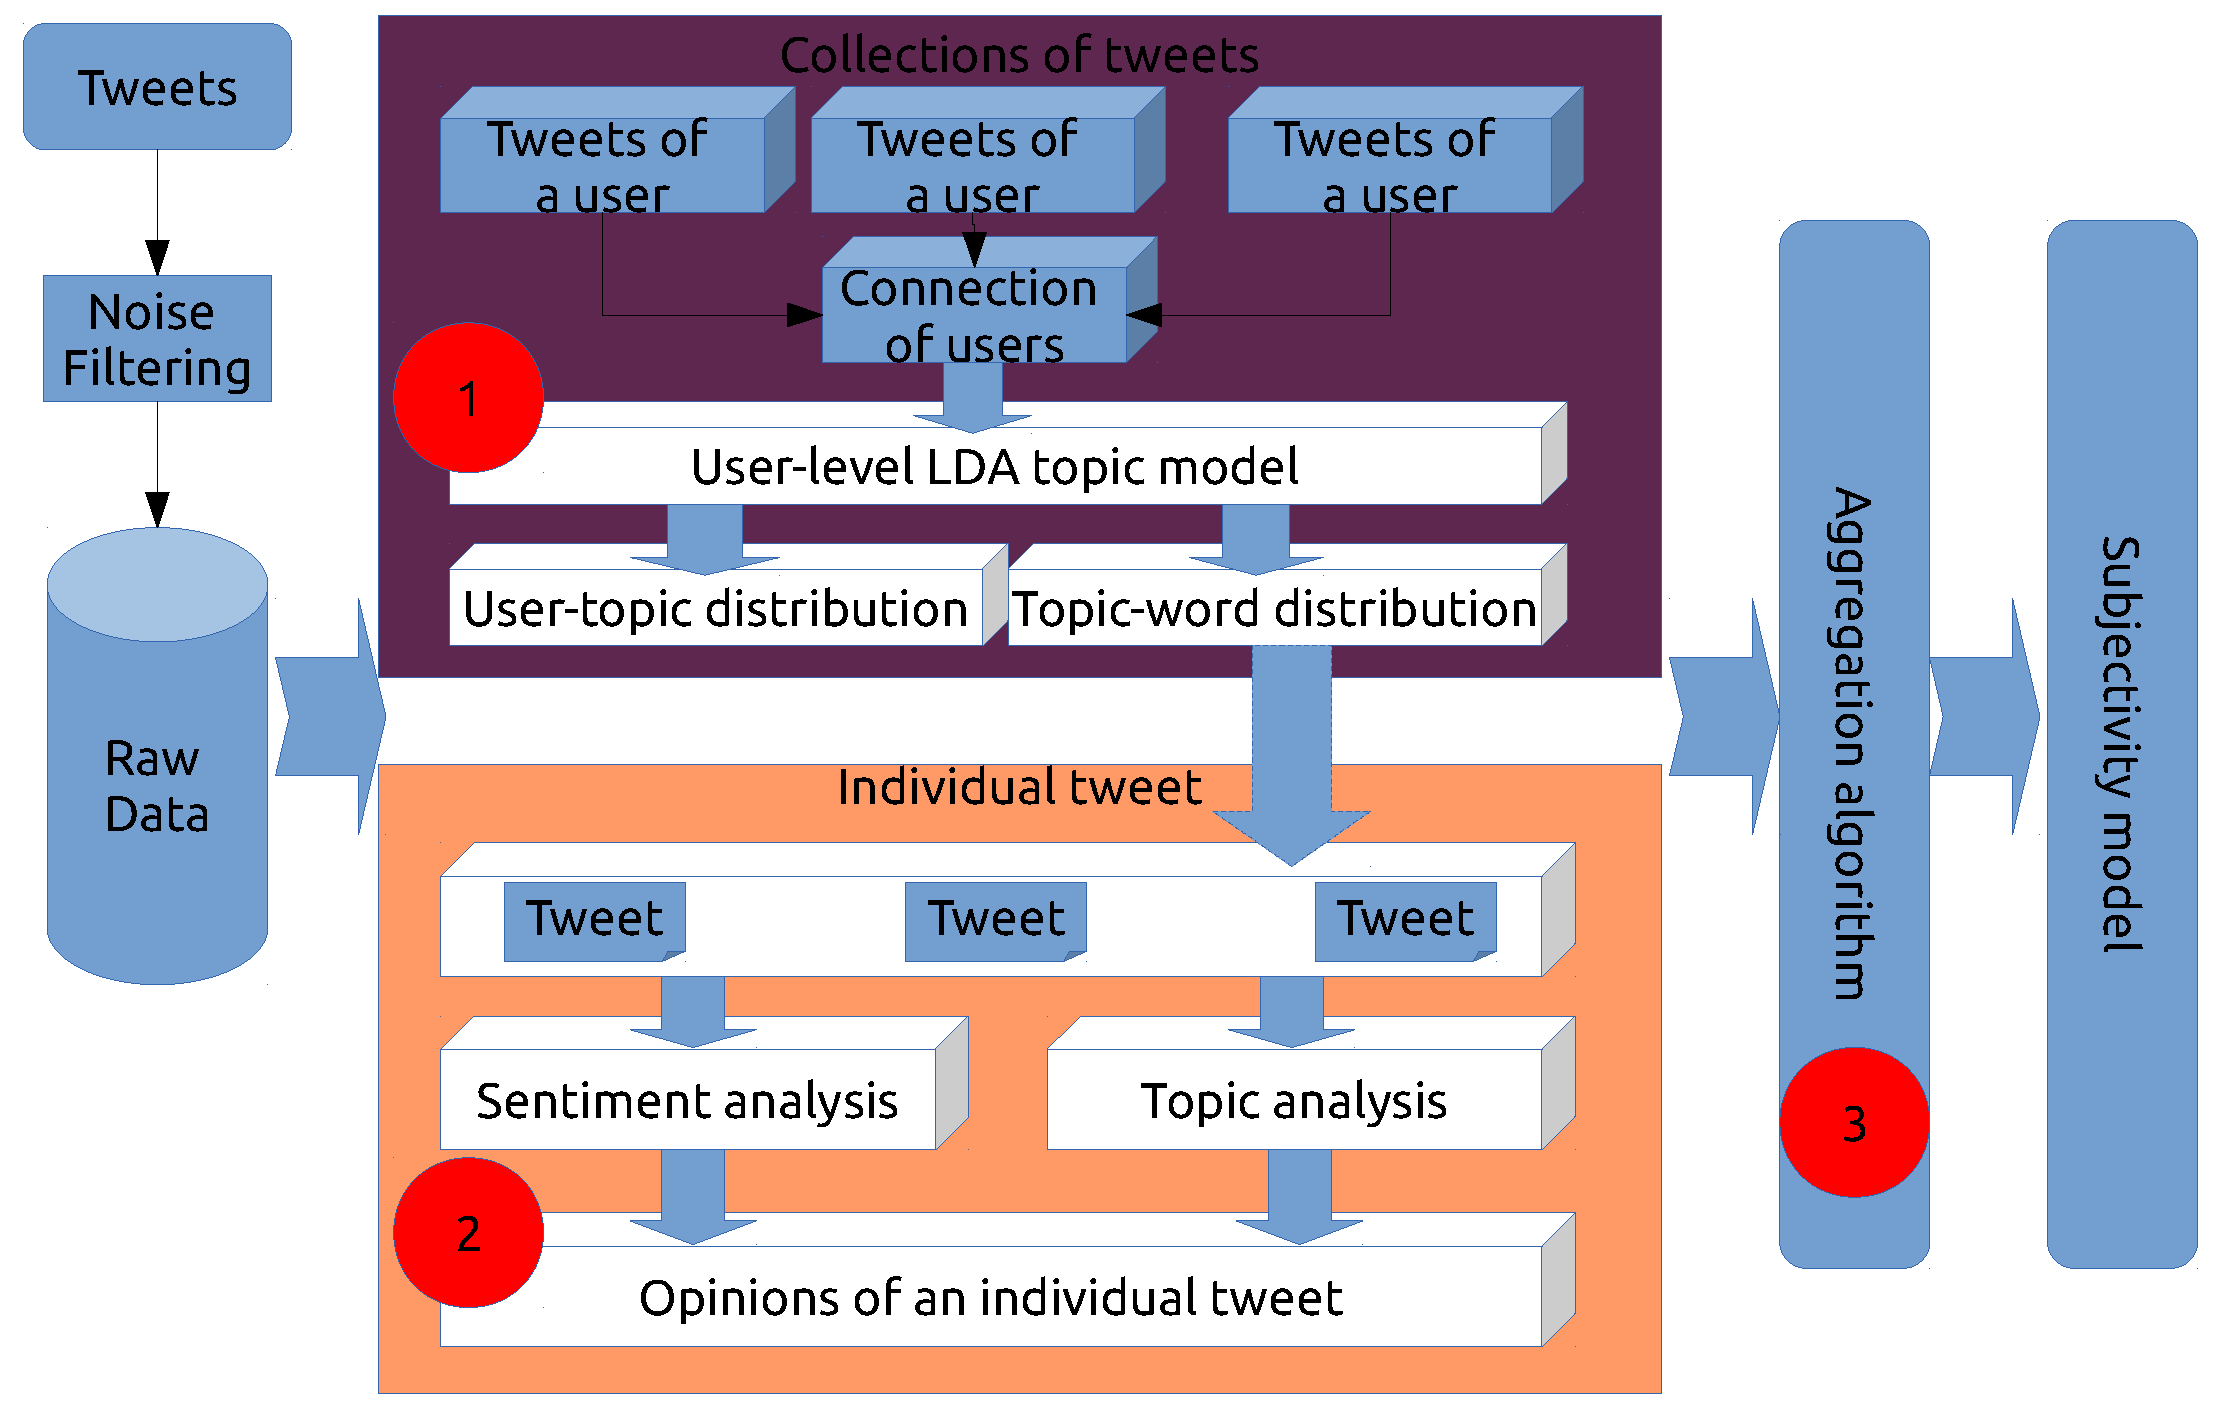
\includegraphics[height=280pt]{5-1.png}
\caption{主观模型总体框架.}
\label{fig5-1}
\end{figure*}
\end{landscape}

\section{相关工作}
\label{ch5_sec2}
虽然观点挖掘(opinion mining)最先是针对产品评论(review)和新闻评论(news comment)\upcite{Pang2008OMS,Liu2012},近年来越来越多的研究工作开始关注于Twitter等短文本社交媒体,主要是针对单个短文本进行情感分析\upcite{Barbosa2010,Davidov2010,Jiang2011,Li2010,tan2011user},往往忽视了用户之间与数据之间的关系。也有一些前期工作研究自动挖掘用户层次的主观性信息\upcite{Mostafa2013,Malouf2008},通常是着眼于识别用户发表观点的目标\upcite{Liu2010}或是针对特定目标确定用户的情感倾向性\upcite{Zhai2011},而没有考虑到话题的每个方面(aspect)。自从Blei等\upcite{Blei2003}发表了潜语义话题模型(Latent dirichlet allocation,LDA),已经有了各种扩展的LDA模型用于从大规模语料中抽取用户的话题\upcite{Rosen-Zvi2004,Ramage2009},也有很多模型将情感分析与话题模型想结合形成话题-情感(topic-sentiment model)模型,这种模型将情感倾向与话题关联起来,与我们提出的主观模型很相似,主要有Mei等的TSM模型\upcite{Mei2007}和Lin等的JST模型\upcite{Lin2009}。

随着用户在社交媒体上公开信息的增多,研究者能够获得越来越多的数据对用户建模,通过这些用户模型使得研究用户行为等研究更加容易。Hannon等\upcite{Hannon2010}首先提出使用微博内容以及Twitter的社交网络关系对Twitter用户进行建模。Macskassy和Michelson\upcite{Macskassy2011}使用Wikipedia作为外部知识库确定用户产生内容中的实体来对用户兴趣进行建模。Ramage 等\upcite{Ramage2010}使用4S维度利用话题模型对用户的微博及你想那个分析建模,得到的模型在信息过滤和朋友推荐等应用中显示出了很好的效果。Xu等\upcite{Xu2012}提出了一个混合模型用于分析用户的发帖行为,混合模型将突发新闻、朋友发帖以及用户兴趣三个重要因素结合在一起。Pennacchiotti和Popescu~\upcite{Pennacchiotti2011}提出了一个全面的方法对用户建模用于用户分类任务,确认了从用户产生内容中挖掘深入的特征的价值,方法反映了对用户及其网络结构的深入理解。

上述这些工作都确认从用户自己发布的内容中挖掘关键信息的重要性,并且开始从四方面信息进行建模,即基本信息(“Who you are”),发帖行为(“How
you tweet”),发帖内容(“What you tweet”)以及网络关系(“Who you tweet”),但是很少能够对用户的兴趣和观点进行综合建模,也就是全面反映用户的主观性,本章中我们将提出主观模型对用户的主观性进行综合建模。

\section{观点集成问题}
\label{sec3}
正如我们在引言部分所介绍,用户在使用社交媒体平台的时候通常会就感兴趣的多个话题的多个方面多次发表自己的观点。因此要确定一个用户在某个话题上观点不能只看他的一条微博,应该将他所有与特定话题相关的微博中的主观信息进行综合才能得出用户的真正观点。在本章我们提出观点集成问题(\textbf{Opinion Integration Problem} (OIP))来对用户的主观性进行建模,我们主要关注用户层次(user-level)观点信息,而不是单个微博层次(tweet-level)的观点信息,因为观点挖掘的最终目标是找到人的主观想法而不只是单条微博中的主观信息,而对单条微博中观点的挖掘只是对用户主观性建模的一个中间步骤。此外,很多情况下用户的单条微博中的观点信息因为受到长度限制以及上下文语境的缺失是不明确的,但是通过看用户的所有微博就可以知道他的明确的观点\upcite{tan2011user}。

我们所提出的话题相关的观点集成问题(OIP)可以使用图~\ref{fig5-2}进行说明。
\begin{figure}[htb]
\centering
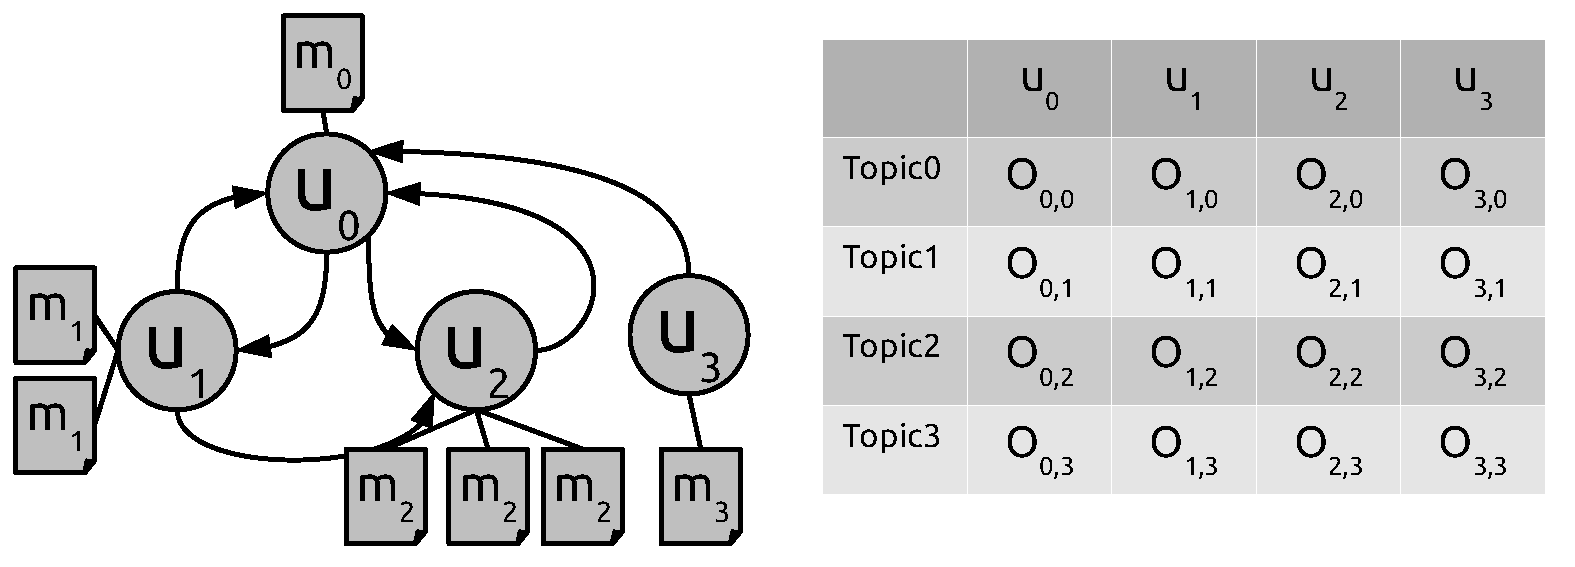
\includegraphics[height=150pt]{5-2.png}
\caption{观点集成问题示例。}
\label{fig5-2}
\end{figure}

我们给出观点集成问题的正式定义:

\begin{definition}[观点集成问题]
如图~\ref{fig5-2}所示,假设Twitter上的一个异构网络(heterogeneous network)由用户集$ V=\left\{ u_{i} \right\} $,用户关系集合$ E=\left\{(u_{i},u_{j})| u_{i},u_{j} \in V\right\} $以及用户发表的相应微博集合$ M_{i}=\left\{ m_{i} \right\} $构成,其中用户所关注的话题$ T=\left\{ Topic_{j} \right\} $以及用户对话题的观点可以从用户自己发表的微博中确定和抽取出来。对于一个特定用户$ u_{i} $,其对特定话题 $ Topic_{j} $的观点$ O_{i,j} $不是他某条微博$ m_{i} $中包含的观点,而应该是从他所有微博中与话题$ Topic_{j} $相关的所有微博$ M_{i}=\left\{ m_{i} \right\} $中集成得出的。
\end{definition}

对观点集成问题有两点因素必须考虑:首先为了观点针对目标的一致性,异构网络中无论是用户还是微博谈及的话题必须是在同一个话题空间,以使得无论话题的表示形式(比如概念(concept)表示或是话题模型的词袋向量空间的多项式分布表示)还是粒度都能够标准规范;其次,也是最重要的,就是集成的观点的表示形式问题,由于观点是与话题紧密相连的,一个用户针对某话题所发表的所有微博会覆盖与话题相关的所有方面,并且对于不同的方面会有不一样的喜好,比如对于手机“iphone”,用户可能喜欢它好看的外观和智能化操作系统,却不喜欢电池的待机时间过短,因此采用什么样的形式表示集成后的观点能准确表达出用户的总体主观性是一个十分重要的问题。本章中我们提出一个全新的通用主观模型来满足以上两个因素。

\section{主观模型}
\label{sec4}
心理学已经对主观性进行了广泛的研究,并基于用户的历史行为和言论中体现出的主观性来表示其独特个性\upcite{Engbert2007}。在语言学上,语言中的主观性定义为作者在其发表的文本中表现出自己的立场、态度和情感\upcite{Stein2005}。社交媒体的出现为用户提供了能够及时自主针对感兴趣话题表达自己意见以展现自己独特主观性的发帖平台,因此在社交媒体平台上,用户的”\textbf{主观性}“,我们定义为用户产生内容中话题和针对话题的观点,因为主观性不但涉及到观点信息,也应该包含观点的目标。

在这一节,我们首先给出主观模型的形式化定义以满足提出的观点集成问题的需求。一般来讲,用户层面的观点分析是将用户针对某话题的情感倾向性分为“正面的(positive)”或是“负面的(negative)”。“正面的“表示该用户对话题支持或者喜欢该,而“负面的”表示不支持或不喜欢。我们所提出的主观模型中采用了更加通用(general)的“观点”定义,也就是观点针对某话题观点是在一个带有情感强度的更细粒度的情感表达空间里的情感分布,这个细粒度的情感表达空间可以更好的区分细微的观点差别,比如对话题持支持度为8的观点比支持度为5的观点更加“正面(positive)“。其实对观点的定义还没有统一的标准,我们采用这种比较广义的定义是为了能使得我们的模型能够更加通用。本章中为了具体化,我们统一在Twitter平台对主观模型进行定义和讨论,其实该模型可以适用于其他的平台或媒体。之所以将模型命名为”\textbf{主观模型}“是因为它是对社交媒体中用户产生数据中的主观性信息进行建模。模型的定义如下:

\subsection{模型定义}
\label{definition}
假设$G=\left( V,E \right) $表示Twitter上某个异构社交网络,其中$ V $是网络中的用户,$ E\subset V\times V $是用户之间的关注关系(follow relationship)。对于每一个用户$ u \in V $,对应的微博集合 $ M_{u} $表示其发帖的历史。可以认为在这个社交网络中存在一个话题空间$ T $ 包含了$ V $中所有用户谈论的所有话题,以及某个情感强度值空间$ S $用于表示用户对某话题的观点。
对于用户$ u  \in V $的”\textbf{主观性(subjectivity)}“,指的是用户所发表的微博$ M_{u} $中所涉及的所有话题以及观点。
  
\begin{definition}[主观模型]
用户$ u $的主观模型$ P \left( u \right) $是用户在话题空间$T$中所谈论话题$\left\lbrace  t \right\rbrace $以及他对每个话题所持有的观点$\left\lbrace O_{t}\right\rbrace $,观点用情感强度空间$ S $的情感分布表示。
\begin{equation}
\label{usermodel}
P \left( u \right) = \lbrace \left( t, w_{u} \left( t \right), \lbrace d_{u,t} \left( s \right)|s \in S \rbrace \right) |  t \in T \rbrace
\end{equation}
其中:
\begin{itemize}
\item 对于用户$ u $,权重$ w_{u} \left( t \right)$表示其在话题空间中每个话题$t \in T$的兴趣强度,并且$ \sum_{t=1}^{|T|}w_{u} \left( t \right)=1 $。
\item 用户$ u $对每个话题$t$的观点$O_{t}$指其对话题所持情感在情感强度空间$ S $的分布$O_{t}=\lbrace d_{u,t} \left( s \right)|s \in S \rbrace $,并且$ \sum_{s=1}^{|S|} d_{u,t} \left( s \right)=1$。
\end{itemize}
\end{definition}

主观模型通过将用户感兴趣话题与观点同时考虑对用户的主观性进行建模,用户兴趣使用一个话题分布表示,对话题的观点用一个情感强度分布表示,主要目标是为了研究用户层面的观点信息,获得用户兴趣和主观思想的比较全面理解。

\subsection{主观模型的构建}
\label{establish}
根据主观模型的定义,我们使用了两个分布对用户的主观性进行建模:一个是话题分布,一个是针对每个话题的观点分布,二者都需要从用户发布的历史数据中经过计算推断得出。然而对Twitter数据进行内容分析面临一些挑战:Twitter上微博数量十分巨大,但是每条微博由于受限于140字的限制而很短小,并且各种不规范的语言被广泛使用,这些都很容易使得机器学习方法和自然语言处理技术失效\upcite{cambria2014jumping}。
因此能够有效的对Twitter的数据内容进行建模处理需要一些能适应这些挑战并且尽量不使用有监督的方法技术。本章中,我们主要使用一些无监督的方法从用户产生数据中挖掘话题和观点信息来构建用户的主观模型。我们提出了一个通用的框架来构建主观模型,该框架的主要优势就是利用Twitter的社交网络结构来帮助客服微博短文本造成的稀疏问题以及微博中标注数据的不足\upcite{Lin2010}。

\subsubsection{话题分析}
\label{topic}
微博所涉及的话题一般是隐含的需要从其内容中推导得出。先前的研究主要是通过找到关键词(key words)\upcite{Chen2010},抽取实体(extracting  entities)\upcite{Abel2011},链接到外部知识库(external knowledge categories)\upcite{Macskassy2011},或者使用语义框架(semantic framework)\upcite{Gangemi2014}。对于这些方法来说,一个主要的问题是稀疏问题,因为同样涉及到同一个话题用户人然会使用各种不同的词汇来表达。在话题模型出现后,对于LDA\upcite{Blei2003}及其扩展的研究工作\upcite{Weng2010}显示出对微博语料更加有效。LDA的话题在概念上更加宽泛,因为LDA的每一个话题都是由所有相关的词语所构成。因此我们采用了用户层面(user-level LDA)话题模型来从用户所有的微博中发现隐含的话题,该模型的生成过程可以使用图~\ref{fig5-1}来示意。

\begin{figure}[htb]
\centering
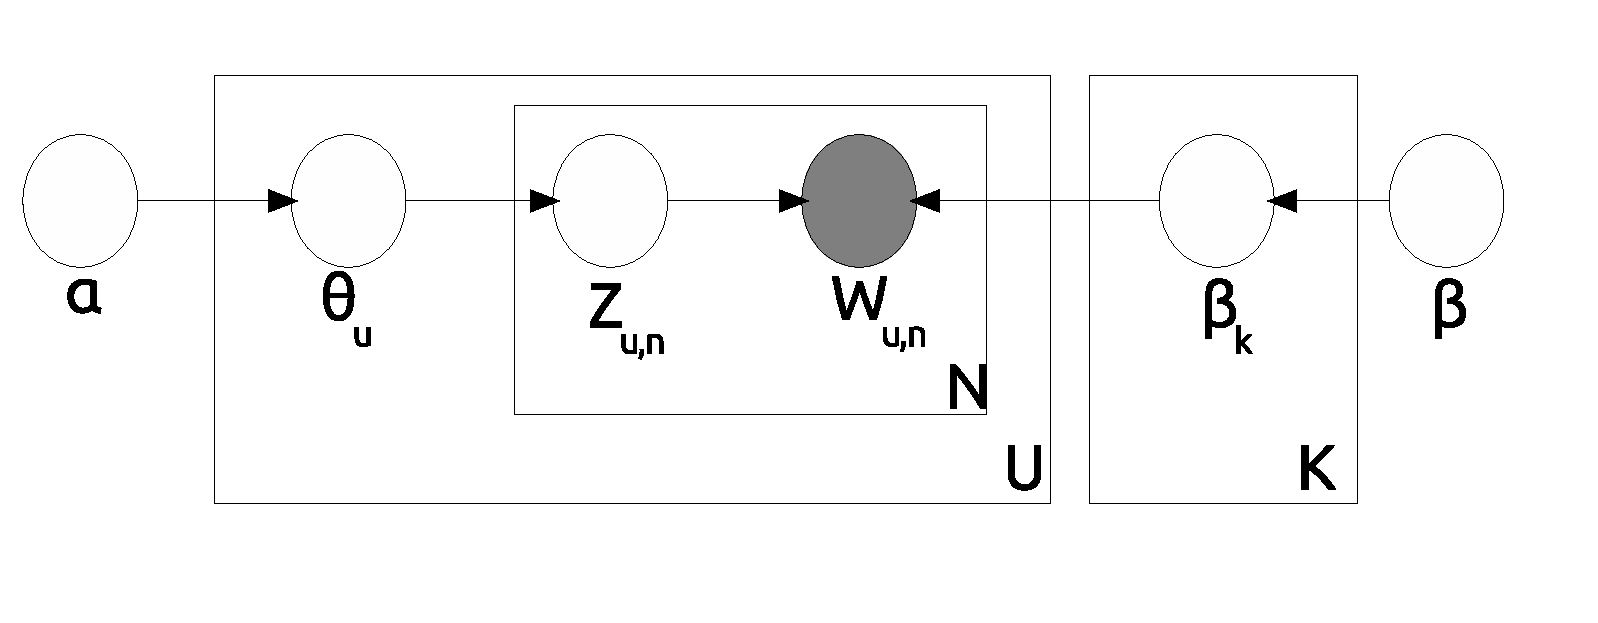
\includegraphics[height=80pt]{5-0.eps}
\caption{用户层面LDA话题模型}
\label{fig5-1}
\end{figure}

生成过程如下:
\begin{itemize}
\item 对每个用户$ u $, 获取话题分布$ \theta_{u} \sim Dir \left(  \alpha \right) $;
\item 对用户微博中的每个词语$ w_{u,n} $,$ n \in \left\lbrace 1, \cdots, N \right\rbrace $:
\begin{itemize}
\item 获取一个话题$ z_{u,n} \sim Multinomial \left( \theta_{u}  \right) $;
\item 基于话题$ z_{u,n} $,从话题的多项分布中获取词语$ w_{u,n} $:\\ 
$$  p \left( w_{u,n} \vert z_{u,n}, \beta_{k}  \right) $$;
\end{itemize}
\end{itemize}

为了从用户产生的内容中提取出讨论的话题,用户所发的微博应该和LDA模型的文档自然对应起来。由于我们的目标是了解用户感兴趣的话题而不是单条微博谈论的话题,所以我们将一个用户所有的微博连接起来组成一篇大的微博文档作为LDA 模型的文档。因此LDA模型中的一篇文档就对应于一个用户,因此一个用户感兴趣的话题就可以使用在话题空间的一个多项式分布来表示,正好可以和我们的主观模型的话题权重相对应。在用户层面的LDA模型中,给定用户集合$ V $以及话题数目$ K $,一个用户$ u \in V $的所有微博文档可使用话题上一个多项分布$ \theta_{u} $来表示,该分布具有参数为$ \alpha $的Dirichlet先验分布;一个话题$ k \in K $可以用所有词汇上的一个多项分布$ \beta_{k} $来表示,该分布具有参数为$ \eta $的Dirichlet先验分布。模型中的两个分布能够使用Gibbs采样或变分推理(variational inference)进行估计。本章中我们使用的是基于变分推理的话题模型工具Gensim\upcite{vRehruvrek2010},该工具使用的是在线批处理模式的变分推理,而且能够对新文档进行话题推理。

\subsubsection{观点分析}
\label{sentiment}
微博用户经常会通过发表一些跟自己感兴趣话题相关的微博来表达自己的观点,因此为了挖掘微博用户的主观信息,我们需要了解用户每条微博蕴含的情感倾向,这需要情感分析技术。情感分析主要有基于规则以及机器学习两种方法。机器学习的训练过程需要大量标注数据,因为Twitter的庞大的数据量以及语言的动态性不太可能达到这样的要求,因此我们采用基于规则的方法,基于规则的方法具有很好的灵活性,可以将Twitter语言的一些特点转换成为规则而更适用于Twitter\upcite{Hu2013,Thelwall2010}。

SentiStrength是专门针对社交媒体中的不正规短文本进行情感分析的工具包\upcite{Thelwall2010}。SentiStrength将对应于社交媒体语言的规则结合进了基于词典的方法,非常适用于我们能够对微博进行情感分析的要求。SentiStrength对每条微博情感分析后赋予两个情感值:一个正面情感倾向强度值(在$ [1,5] $范围内)和一个负面情感倾向强度值(在$ [-5,-1] $范围内)。SentiStrength情感分析的输出不是简单的正负倾向二值结果,而是细粒度的情感强度值,正好符合主观模型能够获得细粒度情感空间上情感分布的需求。为了计算的方便,我们将SentiStrength的两个输出结果映射为一个值,使用$ [0, 8] $的离散整数值表示情感的强度,映射函数为:

\begin{equation}
\label{opinionmap}
o=\begin{cases} 
{p+3} &  \qquad if \; \vert p \vert > \vert n \vert \\
{n+5} &  \qquad if \; \vert n \vert > \vert p \vert \\
{4}  &   \qquad if \; \vert p \vert = \vert n \vert
\end{cases}
\end{equation}
其中$ p $代表SentiStrength输出的正面情感倾向值,$ n $代表负面情感倾向值。在$ [0, 8] $情感空间中,强度值4和5表示中性(neutral)情感,强度值大于5表示正面情感倾向,强度值小于4表示负面情感倾向。使用SentiStrength对用户的每条微博进行情感分析后,就可以$ [0, 8] $情感空间内在进行观点的集成了。

\subsubsection{构建主观模型}
\label{concrete}
对用户微博进行话题分析以及情感分析后,我们就可以为用户开始构建主观模型了。
对于一社交网络的用户集合$ V $,用$ M_{u}=\left\lbrace m_{i} \right\rbrace$表示每一用户 $ u \in V $所发布的所有微博。按照用户层面LDA话题模型要求,将$ M_{u} $中所有微博连接在一起形成一片长的微博文档$ d_{u} $,然后可以用这些微博文档$\{ d_{u}|u \in V\} $使用LDA话题模型进行训练获得话题个数为$ K $的话题空间。
训练得到的话题模型用参数$ \theta $表示每个用户在话题空间$ T $中感兴趣的话题的分布,参数$ \beta $表示每个话题在所有微博词汇上的分布。
使用SentiStrength对每个用户的每条微博$ m $进行情感分析得到每条微博大的情感强度$ s_{m} $。
于是对用户$ u $构建主观模型$ P(u) $的过程如算法~\ref{alg5-1}所示:

\begin{algorithm}[htb] 
\caption{主观模型的构建过程} 
\label{alg5-1}
\begin{algorithmic}[0] %这个1 表示每一行都显示数字
\REQUIRE ~~\\ %算法的输入参数:Input
The users set of a local network, $ V $;\\
The tweets set published by each user $ u $, $ M_{u} $;\\
\ENSURE ~~\\ %算法的输出:Output
The subjectivity model for each user $ u $, $ P(u) $;
\STATE Topic analysis with a user-level LDA, getting a topic model $P(\theta,\beta|M_{u},V)$; 
\label{ alg1:topic }%对此行的标记,方便在文中引用算法的某个步骤
\FORALL {tweet $ m \in M_{u} $}
\label{alg1:sentiment}
\STATE Sentiment analysis, outputting sentiment of $ m $, $ s_{m} $;
\ENDFOR
\FOR {user $ u \in V$}
\STATE the topic distribution is the corresponding component of parameter $ \theta $, $ \theta_{u} $; \\
\STATE the topics he tweets about are $ Z_{u}= \left\lbrace t \vert p\left( t \vert \theta_{u} \right)>0, t \in T \right\rbrace $; 
\ENDFOR
\FOR {tweet $ m \in M_{u} $}
\STATE topics of $ m $ can be identified by the topic model:
\begin{equation}
\label{tweettopic}
Z_{m} =\left\lbrace t \vert p\left( t \vert \theta, \beta, Z_{u} \right)>0, t \in T \right\rbrace.
\end{equation}
\ENDFOR
\FOR { each topic $ t \in Z_{u} $ }
\FOR { sentiment value $ s \in S $}
\STATE count the number of tweets which talk about topic $ t $ with sentiment value $ s $: $ N_{s}=\sum_{m \in M_{u}} I\left( s_{m} \right) ,  if  s_{m}=s \& t \in Z_{m} $;
\ENDFOR
\STATE calculating opinion towards topic $ t $: $ O_{t} = \left\{ \frac{N_{s}}{\sum_{s \in S} N_{s}} |s \in [0,8] \right\}  $.
\ENDFOR
\STATE establishing subjectivity model of user $ u $:
\begin{equation}
\label{subuser}
P\left( u \right)= \left\lbrace \left( t, p\left( t \vert \theta_{u} \right), \left\{ \frac{N_{s}}{\sum_{s \in S} N_{s}} \right\}  \right)  \vert t \in Z_{u}, s \in S  \right\rbrace.
\end{equation}
\RETURN $P(u)$; %算法的返回值
\end{algorithmic}
\end{algorithm}

算法中,由于微博的短小,我们简单假设微博$ m $的情感$ s_m $是针对微博所讨论的所有话题$ Z_{m} $的,并没有区分针对不同话题的不同观点。

\subsection{与生成模型比较}
\label{comparison}
前期研究中提出了一些基于话题模型的生成模型,能够扩展基本的话题模型将文档中表达的情感与话题结合统一建模\upcite{Mei2007,Lin2009}。TSM模型(Topic Sentiment Mixture model)\upcite{Mei2007}认为文档中表示情感等主观信息的语言与描述话题的语言是独立的,因此可以将表示情感的语言模型跟表示话题的语言模型分开,在文档的生成过程中词语要么从话题中要么从情感中采样获得。JST模型(Joint Sentiment/Topic model)\upcite{Lin2009}提出了一种新的方式来分析文档中的情感信息,使用话题模型抽取话题过程中将话题和情感关联起来,因此可以同时对话题和情感信息建模。
这些模型在发现话题相关的观点信息时跟我们提出的主观模型是很相似的,都能同时对用户的感兴趣话题以及话题相关的观点建模。

但是他们通常需要通过学习获得一个通用词语-情感分布来对文档中的情感建模,这对短小和不正规的社交媒体语言尤其是Twitter来说是困难的。相较于话题的表达,情感等主观信息更难发现,u因为情感信息常常隐含在一些微妙的语言表达方式中(比如反讽),还有一些具体的领域和语境中也会具有独特的情感表达方式。微博中的情感除了一些正规的表达语言外,还有很多微博特有的语言特色来表示,比如表情符、字母大小写、字母重复以及惊叹号的使用等等。微博上的这些语言特色很难用概率分布来表示用于对情感建模。可是基于规则的情感分析方法可以很容易通过将这些语言特色转化为规则来抓住微博语言中微妙的情感表达方式。因此,我们的模型采用了基于规则的情感分析工具发现微博中的情感信息,更适合于Twitter等短文本社交媒体上用户主观信息的建模。

\subsection{主观模型的应用}
\label{application}
从用户微博中学习得到的主观模型能够在用户观点挖掘分析以及行为分析预测(转发、关注等行为)得到应用。本章我们以用户观点的预测为例来验证主观模型的作用,也就是学习到的主观模型能否有效的对用户将来针对某话题的观点进行预测。根据据用户观点的一致性,我们认为用户不会就某一话题表达随机正面或负面的观点,例如按照常理一个支持某候选人的用户更趋向于针对该候选人发表正面观点的微博。社会学上称这种现象为人的主观偏执(bias),也就是人的主观性\upcite{Walton1991}。因此得到了用户的主观模型,就可以预测用户就某一话题发表的微博所持观点。

我们将观点预测问题形式化为三元组$ < author, m, t >$,其中$author$微博$ m $作者,微博涉及话题为$ t $。观点预测的目标就是计算得出用户$author$的微博$ m $针对话题$ t $表达出的观点极性$ p=\left\{positive,negative\right\} $。情感分析领域针对这一问题的主要方法是从微博中抽取出文本的表达模式,然后探索这些模式来预测观点的极性。
单条短微博经常会由于缺乏上下文信息而使得观点模糊不清,但是用户的主观模型是从用户所有的微博中建立的,因此具有足够的信息,并且由于用户主观性的一致性,主观模型的观点信息比一条短文本更加可靠。因此我们提出使用主观模型来提高观点预测效果。
具体来说,对微博$ m $,其作者的主观模型算法~\ref{alg5-1}构建,微博$ m $的情感值通过某种方法比如SentiStrength得出为$s_m$。微博$ m $所谈论的话题可以使用的公式~\ref{tweettopic}推导得出:

\begin{equation}
\widehat{t}=argmax(\widehat{P}(t| \theta,\beta ,Z_{u})|t).
\end{equation}
用户$author$的观点分布可以从主观模型$ P(author) $中确定,$ O_{author,\widehat{t}} $,为在情感值上的分布,我们可以计算出用户在话题$ \widehat{t} $上归一化情感值:

\begin{equation}
\widehat{s_{m}}=\sum_{i \in T}d_{i}\ast v_{i}
\end{equation}
其中$ v_{i} $表示情感值,$ d_{i} $表示情感值对应的分布。
于是可以使用微博的情感值$s_m$和归一化的主观模型情感值$ \widehat{s_{m}} $进行观点极性$ p $预测:

\begin{equation}
\label{polarity}
p=  
\begin{cases}
{positive} &  \qquad if \; \dfrac{\widehat{s_{m}+s_m}{2}} > \dfrac{|S|}{2} +1\\
{negative} &  \qquad if \; \dfrac{\widehat{s_{m}+s_m}{2}} < \dfrac{|S|}{2} \\
{neutral}  &   \qquad otherwise \;  
\end{cases}
\end{equation}
其中$ S $是情感强度空间。

\section{实验}
\label{sec5}

\subsection{数据集及设置}
我们使用的是通过Twitter公开的API抓取的现成的数据集\upcite{Li2012a}。数据集的具体细节在表~\ref{tab5-1}中列出。

\begin{table}
\centering
\caption{Twitter数据集统计}
\label{tab5-1}
\begin{tabular}{ll|ll}
\hline
Total users  & 139,180 & Friends per user & 14.8 \\
Total edges &  4,175,405 & Followers per user & 14.9  \\
Total tweets & 76,409,820 & Tweets per user & 549 \\
\hline
\end{tabular}
\end{table}

由于LDA模型的计算复杂度,直接从139,180个用户的所有微博中构建主观模型需要耗费大量的时间。根据社交网络的同质性\upcite{Lazarsfeld1954},也就是“物以类聚(birds of a feather flock together)”的原则\upcite{McPherson2001},社交网络中连接紧密的用户更趋向于讨论形同话题持有相似观点\upcite{Thelwall2010a}。在Twitter上,用户之间的连接关系对应着认可或关注,或者意味着有相似话题或观点。因此我们利用社交网络的社区结构(community)将139,180个用户划分为不同的社区,在社区内部为用户构建主观模型。社区的划分我们使用的是
Igraph\footnote{\url{http://igraph.org/}}工具包,最后将用户划分为106个社区。对于用户数少于15的小社区,使用LDA进行话题分析效果比较差,因此我们将这些社区和用户过滤掉。同时我们也过滤掉了发微博少于5的、每次发微博字数少于3个的或微博中只有网络连接的用户15,756个。最后形成的数据集中有122,329个用户,分部于33个社区中。我们为每个用户在其社区内局部网络中按照算法~\ref{alg5-1}构建主观模型。

除了主观模型,我们也使用生成模型JST和TSM进行了对比试验。其中模型的Dirichlet先验参数设为$ \alpha=50/T $($ T $为话题数目),$ \beta=0.01 $。JST的不对称情感先验参数$ \gamma $依照经验设为$ (0.01, 1.8) $。两个模型推导都进行2,000次迭代Gibbs采样。

\subsection{样例分析}
为了定性展示我们所提出的主观模型的有效性,我们给出了一个学习得到的用户的主观模型如图所示。该用户发表了533条微博,所有微博用词云图~\ref{fig5:a}来显示。

\begin{figure}[htb]
\centering
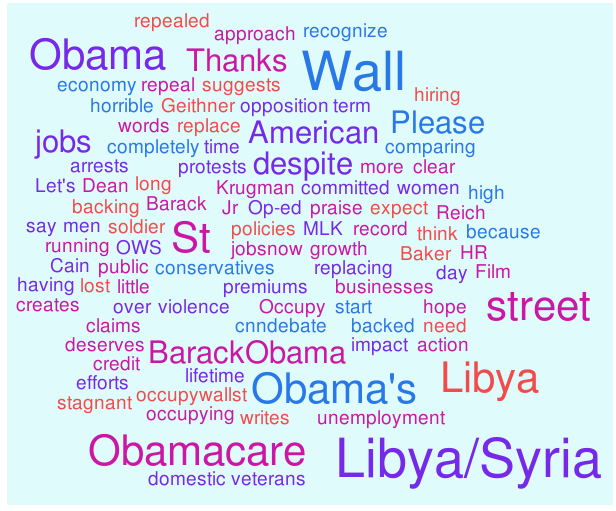
\includegraphics[height=200pt]{5-4.png}
\caption{微博词云}
\label{fig5:a}
\end{figure}

\begin{figure}[htb]
\centering
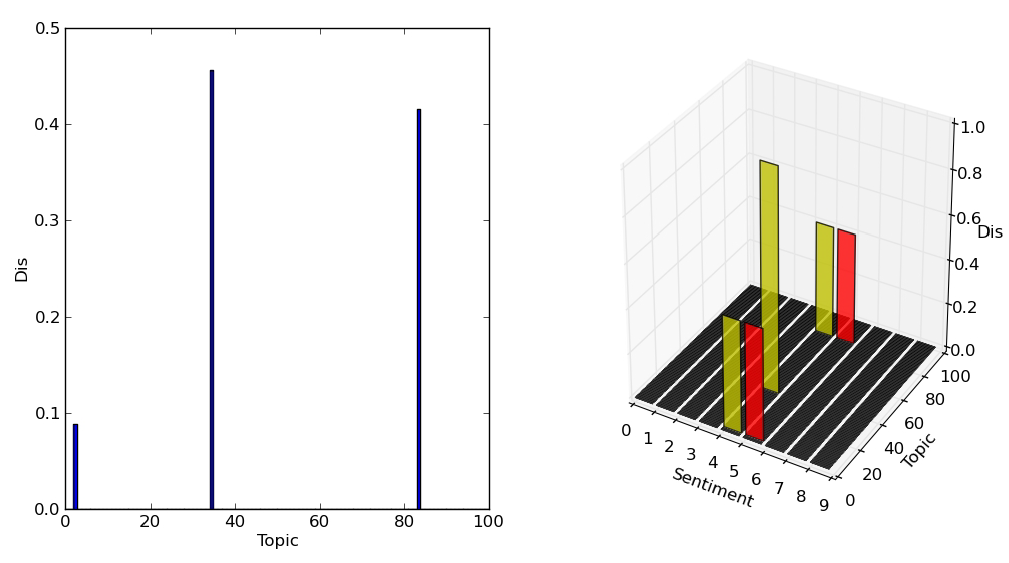
\includegraphics[height=200pt]{5-3.png}
\caption{主观模型。主观模型中,左侧图代表话题分部: $ (  w_{u}\left( 2 \right)=0.08,w_{u}\left( 32 \right)=0.48, w_{u}\left( 83 \right)=0.44)  $;右侧图代表观点的分部: $ O_{2}=( d_{u,2} \left( 4 \right)=0.5, d_{u,2} \left( 5 \right)=0.5)$, $O_{32}=(d_{u,32} \left( 4 \right)=1.0) $, $ O_{83}=( d_{u,83} \left( 4 \right)=0.5, d_{u,83} \left( 5 \right)=0.5 ) $。}
\label{fig5:b}
\end{figure}

图~\ref{fig5:b}是用户在$ [0,100] $话题空间和$ [0,8] $情感强度空间的可视化的主观模型。很明显,从词云图上可以看到该用户讨论了三个话题(话题2:``\#Obamacare'',话题32:``\#libya''以及话题83:``\#occupywallst''),子图~\ref{fig5:b}左侧展示了用户在每个话题上的兴趣权重。子图~\ref{fig5:b}右侧是用户对这三个话题所持观点分布,总体来看,对于话题``\#libya''情感分布100\%在强度4上,属于中性,对话题``\#Obamacare''和``\#occupywallst''情感分部都是50\%在强度4以及50\%在强度5上,属于中性偏正面倾向。从这个样例可以看出,我们的主观模型对用户的主观性进行了详细的建模,不但有用户的兴趣分布,也有细粒度的观点分部信息。

\subsection{观点预测性能}
为了定量评价主观模型的有效性,我们将主观模型在观点预测任务上与两个生成模型(TSM and JST)和一些主流的情感分析方法进行了对比实验。由于缺少可用的标注数据,我们主要跟几个无监督的情感分析方法进行了对比,这些方法主要有:
\begin{itemize}
\item \textbf{OF:OpinionFinder}是一个公开可用的情感分析软件包,主要是用于句子层面的主观性分析\upcite{Wilson2005}。
\item \textbf{S140:Sentiment140}使用远距离监督(distant supervision)方式(使用表情符获取训练数据)进行微博的情感分类。
\item \textbf{STR:SentiStrength}将微博中的一些语言特点转化成规则结合基于词典的方法专门针对微博等短文本社交媒体进行情感分析\upcite{Thelwall2010}。
\end{itemize}

我们从数据集中随机选择了1,000个至少有80条微博的用户条,然后每个用户随机选择一条微博组成了1,000条微博的数据集用于性能评测。为了能更容易识别微博的话题,我们优先选择带hashtag的微博。所有的1,000条微博进行人工标注作为评测标准。话题模型的话题数分别设置为50, 100, 150以及200,评价指标使用的是准确率,结果如表~\ref{tab5-2}所示。

\begin{table}[htb]
\centering
\caption{评价结果。相对于OF显著的性能提升使用$ \ast $标记。}
\label{tab5-2}
\begin{tabular}{l|llll}
\hline
Method & 50 & 100 & 150 & 200\\
\hline
OF &  65.85\%& & & \\
S140 &  70.45\%& & & \\
STR &  69.98\%& & & \\
TSM & 63.46\%& 72.94\% $ \ast $  &67.83\% & 66.65\% \\
JST & 61.25\% & 68.57\% $ \ast $ & 75.88\%  $ \ast $ & 67.03\%\\
SUB & 71.53\% $ \ast $ & 81.05\% $ \ast $ & 78.32\% & 74.54\%\\
\hline
\end{tabular}
\end{table}

从表中可以看出:

首先,OpinioFinder的准确率是最低的65.85\%,主要原因是OpinioFinder主要是针对评论而设计的主观性信息分析工具,不适用于Twitter这种语言环境;

第二点,两个情感分析方法的准确率都显著的好于OpinioFinder(Sentiment140:70.45\%,SentiStrength:69.98\%);

第三点,总体上两个生成模型的准确率都好于OpinioFinder,证明了将情感信息与话题进行关联的重要性,它们的准确率都比Sentiment140和SentiStrength稍好,但是不显著;

最后,我们的模型(SUB)准确率在四种话题设置下都显著地超过了三个情感分析方法,并且将主观模型的信息加入到SentiStrength的分析结果后,显著提高了SentiStrength的性能,与两个生成模型相比较,我们的模型性能明显比TSM要好,稍好于JST,这是因为我们的模型构建所用的情感分析方法更适合与Twitter语言,能够更准确的分析微博中的情感信息。

\section{小结}
\label{sec6}
本章中,我们定义并研究了社交媒体中用户的观点集成问题,提出了主观模型作为解决方案并设计了新的算法来从用户的历史数据中构建主观模型。使用主观模型可以自动总结用户在各个话题上的综合观点。实验证明,主观模型能有效的对用户的主观性进行建模,并且在观点预测任务中基于主观模型的方法性能显著比现有的几个情感分析方法要好,而且比TSM和JST两个生成模型更适于与Twitter。
